\documentclass{article}
\usepackage[utf8]{inputenc}

% 81 column comment
%01234567890123456789012345678901234567890123456789012345678901234567890123456789

% Reduce top margin, increase bottom margin
\usepackage[a4paper, top=3cm, bottom=4cm]{geometry} 
\usepackage{graphicx}		% images
\usepackage{hyperref}

\graphicspath{{images/}}

\title{Final Project\\ CSC410 - Parallel Computing}
\author{Aaron G. Alphonsus}
\date{December 11, 2018}

\begin{document}
\maketitle

\section{The N-queens Problem}
% • Description of the program.

The goal of n-queens problem is to place $n$ queens on an $n \times n$ 
chessboard such that no two queens can attack each other. The queen piece in 
chess can move along rows, columns, and diagonals. This means that any solution 
we find will not have two queens in the same row, column, or diagonal.

\medskip
\noindent
Since no queen can be in the same row or column, we will represent all these 
solutions as an n-tuple $(x_1, x_2, ... , x_n)$ where column 1 has a queen in 
row $x_1$, column 2 has a queen in row $x_2$, $...$, and column $n$ has a queen 
in row $x_n$. With this representation, there are $n!$ possible solutions. For 
each of these solutions, all we need to check is if there are two queens that 
are on the same diagonal.

% e. Benchmark your code.
\section{Benchmarking}
In order to benchmark our program, we use the \texttt{MPI\_Wtime()} function. 
Along with it, we use the \texttt{MPI\_Barrier()} function for barrier 
synchronization so that we start the timer when all the 
processes are ready to begin execution and stop the timer when they all return. 
We place these functions before \texttt{for} loop that evaluates each 
permutation, and after the \texttt{MPI\_Reduce()} call. 

\medskip
\noindent
Figure \ref{fig:benchmark} is a graph of execution time vs size of the problem. 
We used 65 processes for this. The execution time increases `factorially' since 
for each increase in $n$ by 1, The number of solutions to evaluate is $n!$. 
Initially there isn't much change in total execution time as the problem 
execution time is smaller than the overhead. Once it gets to larger numbers, the
program execution time dwarfs the overhead time.

\begin{figure}[ht]
	\centering
    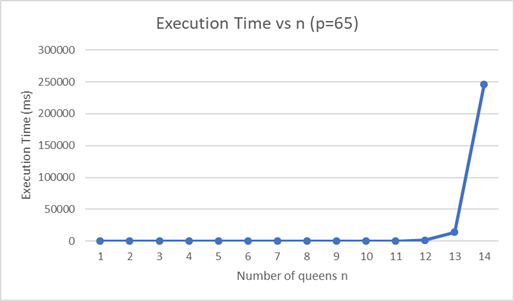
\includegraphics[width=0.6\textwidth]{benchmark.png} 
    \caption{Execution time as problem size increases}
    \label{fig:benchmark}
\end{figure}

% d. Do a complete analysis.
\section{Performance Analysis}
% Some random intro paragraph 
In order to do the performance analysis, we used similar methods to our 
benchmarking step but this time we kept the size of the problem fixed, and 
varied the number of processes. Figure \ref{fig:benchmark_p} shows the decrease 
in execution time with the increase in number of processes. 

\begin{figure}[ht]
	\centering
    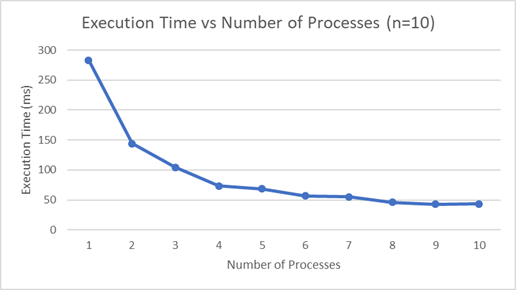
\includegraphics[width=0.6\textwidth]{benchmark_p.png} 
    \caption{Execution time as number of processes increase}
    \label{fig:benchmark_p}
\end{figure}

\medskip
\noindent
In our performance analysis we also calculated the speedup, efficiency, 
Karp-Flatt Metric, and isoefficiency relation. Using the experimentally 
determined serial fraction $f_e$ from the Karp-Flatt Metric, we calculate the 
scaled-speedup. Amdahl's Law yields the same value as speedup when we use $f_e$ 
in our calculation.

\subsection{Speedup and Efficiency}

The speedup $\psi(n, p)$ is the ratio between sequential execution time and 
parallel execution time.
\[\psi(n, p) = \frac{T(n, 1)}{T(n, p)}\]

\medskip
\noindent
Efficiency $\epsilon(n,p)$ is defined as the speedup divided by the number of 
processors used:
\[\epsilon(n, p) = \frac{\psi(n,p)}{p}\]

\medskip
\noindent
The speedup and efficiency for our program as a function of increasing processes
can be seen in figure \ref{fig:speed_eff}. You can see that we get steady 
speedup initially which starts flattening out towards the end. However, the more
processes we add, the less we utilize them as the efficiency goes down steadily 
with increasing numbers of processes.

\begin{figure}[ht]
	\centering
    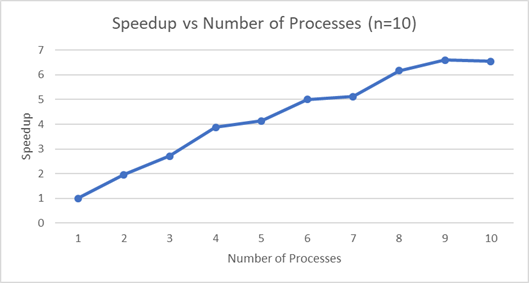
\includegraphics[width=0.45\textwidth]{speedup.png}\quad
    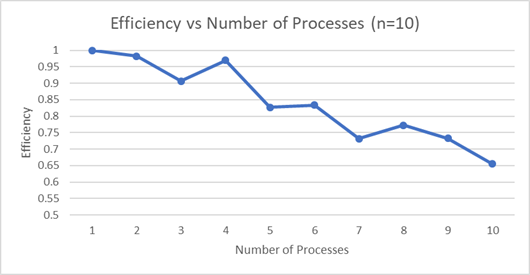
\includegraphics[width=0.45\textwidth]{efficiency.png}\quad
    \caption{Speedup and Efficiency vs Number of processes}
    \label{fig:speed_eff}
\end{figure}

\subsection{The Karp-Flatt Metric}

\medskip
\noindent
The Karp-Flatt metric provides a means to use empirical data to learn something 
about parallel overhead as well as the amount of inherently sequential 
computation in a parallel program. The basic idea is to collect data from 
several runs of the program with increasing numbers of processes.

\medskip
\noindent
\textbf{Definition:} Given a parallel computation showing a speedup $\psi(n, p)$
on $p$ processes, where $p > 1$, the experimentally determined serial fraction 
$f_e$ is defined to be: 
\[f_e = \frac{1/\psi(n, p) - 1/p}{1 - 1/p}\]

\begin{table}[ht]
\centering
\begin{tabular}{|c|c|c|c|c|c|c|c|c|c|}
\hline
$p$ & \textit{2}  & \textit{3}  & \textit{4}  & \textit{5} & \textit{6}  
    & \textit{7}  & \textit{8}  & \textit{9} & \textit{10} \\ \hline

$\psi(n, p)$ & $1.96$  & $2.72$ & $3.88$ & $4.13$ & $5.00$ 
             & $5.12$  & $6.18$ & $6.60$ & $6.55$  \\ \hline

$f_e$ & $0.018$  & $0.052$ & $ 0.011$ & $ 0.052$ & $0.040$ 
      & $0.061$  & $0.042$ & $0.046$  & $0.058$ \\ \hline
\end{tabular}
\end{table}

\medskip
\noindent
What we can see here is that the serial fraction is trending upwards as the 
number of processes increase. This indicates that the main reason for the poor 
speedup is parallel overhead. This could be time spent in process startup, 
communication, or synchronization, or it could be an architectural constraint.

\subsection{Scaled Speedup and Isoefficiency Relation}

\medskip
\noindent
\textbf{Definition:} Given a parallel program solving a problem of size n using 
p processors, The maximum speedup $\psi$ achievable by this program is:
\[\psi \leq p+(1-p) \cdot s\] where s is the fraction of execution time spent in
serial code. We  use the experimentally determined value for the serial fraction
from Karp-Flatt in our calculation of the scaled speedup. Figure 
\ref{fig:scaled_speedup} shows scaled speedup and speedup plotted as a function 
of increasing processes.

\begin{figure}[ht]
	\centering
    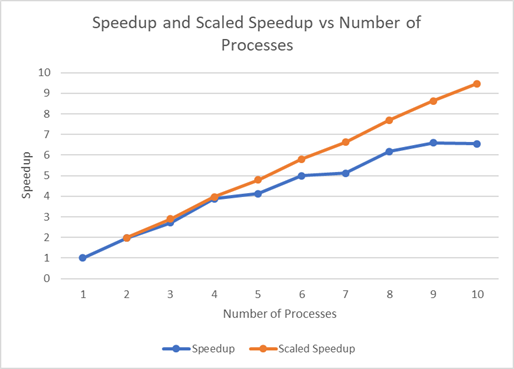
\includegraphics[width=0.6\textwidth]{scaled_speedup.png}
    \caption{Execution time as number of processes increase}
    \label{fig:scaled_speedup}
\end{figure}

\medskip
\noindent
We show the isoefficiency relation for our program graphically in figure 
\ref{fig:isoefficiency}. Notice that C is a lower bound for the fraction 
$T(n,p)/T_0(n,p)$. The isoefficiency relation is the following inequality:
\[T(n,1) \geq C \cdot T_0(n,p)\]
where T(n, 1) denotes the sequential time, $T_0(n,p)$ denotes parallel overhead 
and $C = \epsilon(n,p)/(1-\epsilon(n,p))$

\begin{figure}[ht]
	\centering
    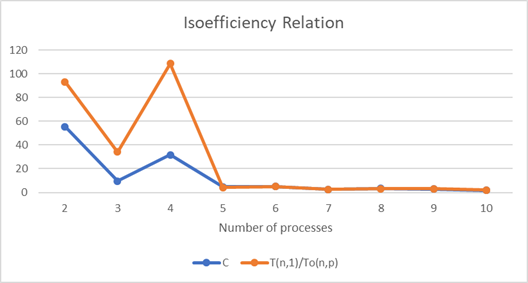
\includegraphics[width=0.6\textwidth]{isoefficiency.png}
    \caption{Execution time as number of processes increase}
    \label{fig:isoefficiency}
\end{figure}

% • Description of the algorithms and libraries used.
\section{Algorithms and Libraries}

To solve this problem we used the Task/Channel model to design a parallel 
algorithm. We began with a cyclic mapping, where the index $i$ of the $n!$ 
possible solutions were given to each process one-by-one. The process would 
calculate the i\textsuperscript{th} permutation of the array $(0, 1, ..., n)$, 
and then test to see if the permutation was a valid solution to place the $n$ 
queens. We knew calculating the i\textsuperscript{th} permutation every time 
couldn't be efficient, so we decided to agglomerate the tasks.

\medskip
\noindent
With this new mapping, each process is given a contiguous chunk of permutations 
to evaluate. This is useful because the \texttt{std::next\_permutation()} 
function in the C++ \texttt{<algorithm>} library is more efficient than 
calculating the i\textsuperscript{th} permutation each time. The first 
permutation is calculated using the \texttt{ithPermutation()} function that we 
wrote, but \texttt{std::next\_permutation()} is used for subsequent 
permutations. 

\medskip
\noindent
Each permutation is then checked to see if it is a valid solution by going 
through every pair of queens and seeing if their row difference is equal to 
their column difference. This would indicate that they are on the same diagonal.
Every process keeps a count of the number of solutions locally. In order to get 
the count of all the solutions, we use the reduction operation 
\texttt{MPI\_Reduce()} to sum up the local sums of each process.

\medskip
\noindent
\subsection{Libraries used}
\begin{itemize}
	\item \texttt{<algorithm>}
    \item \texttt{<math.h>}
    \item \texttt{<mpi.h>}
\end{itemize}

% • Description of functions and program structure.
\section{Functions and Program Structure}

The program has 4 functions:
\begin{itemize}
    \item \texttt{main}
    \item \texttt{usage}
    \item \texttt{ithPermutation}
    \item \texttt{checkDiag}
\end{itemize}

\subsection{\texttt{main}}
Arguments: 
    \begin{itemize}
	    \item \texttt{int argc}: Number of command-line arguments.
        \item \texttt{char* argv[]}: Pointer array storing each command-line 
        argument. 
    \end{itemize}
Returns: \texttt{0} indicating normal termination.

\medskip
\noindent
Description: 
\begin{itemize}
    \item Initializes MPI library, calculates process ranks and total number of 
    processes.

    \item Allocates contiguous chunks of permutation ranges to be checked by 
    each process.

    \item Calculates permutations and calls the solution validation function 
    \texttt{checkDiag()}.
    
    \item Keeps track of the number of local solutions. Performs a reduction to 
    calculate total number of solutions. 
    
    \item Prints out number of solutions and execution time. Prints out 
    solutions if print flag set.
\end{itemize}

\subsection{\texttt{usage}}
Arguments: 
    \begin{itemize}
	    \item \texttt{char* prog\_name}: Character array containing the name of 
	    the program.
    \end{itemize}
Returns: void

\medskip
\noindent
Description: Prints a message explaining how to run the program.

\subsection{\texttt{ithPermutation}}
Arguments: 
    \begin{itemize}
	    \item \texttt{int n}: digits to permute
	    
	    \item \texttt{unsigned long long i}: index of the permutation.
    \end{itemize}
Returns: \texttt{int* perm}: The i\textsuperscript{th} permutation of the array 
$(0, 1, ..., n)$ 

\medskip
\noindent
Description: 
\begin{itemize}
    \item Calculates the factoradic representation of the decimal number i.

    \item Uses the factoradic to obtain the i\textsuperscript{th} permutation.
\end{itemize}

\subsection{\texttt{checkDiag}}
Arguments: 
    \begin{itemize}
	    \item \texttt{int n}: number of queens and size of chessboard.
	    
	    \item \texttt{int perm[]}: Possible solution to be accepted or rejected.
    \end{itemize}
Returns: \texttt{int}: 1 if no queens share a diagonal, 0 otherwise.

\medskip
\noindent
Description: For each pair of queens, check if horizontal distance from each 
other is the same as vertical distance. If so, the queens are on the same 
diagonal.

\section{Compilation and Usage}
Compilation: \texttt{mpiCC -g -Wall -o nqueens nqueens.C -lm} OR \texttt{make} 

\noindent
Usage: \texttt{mpirun -np <num of processes> -hostfile <hostfile location> 
./nqueens <n> <print>}

\medskip
\noindent
The program can be compiled using the command \texttt{make}. To get rid of the 
executable in the folder, run the command \texttt{make clean}.

\medskip
\noindent
The program takes in an integer $n$ indicating number of queens and size of the 
chessboard, as well as a 0 or 1 suppressing or allowing printing of solutions to
the console window. The program prints out the number of solutions and execution
time by default.

\section{Testing and Verification}
% • Description of the testing and verification process.
% c. Complete testing of your code.
For verification, as we built the program we used small values of \texttt{n}
(n=1 to n=6) and printed out the solutions. We found these solutions by hand and
confirmed that they matched the ones we were getting with our program.

\medskip
\noindent
For slightly larger solutions, we sorted our solutions and wrote them out to a 
list. We compared this list with the output of an n-queens program found online 
that we edited slightly to give the same tuple output that we have. 

\medskip
\noindent
For large values of n and large numbers of solutions, we tested our program 
based on getting the right number of solutions (figure \ref{fig:solutions}). We 
decided that the odds that we got the same number of solutions but had a wrong 
solution for multiple values of $n$ was unlikely :) 

\begin{figure}[ht]
	\centering
    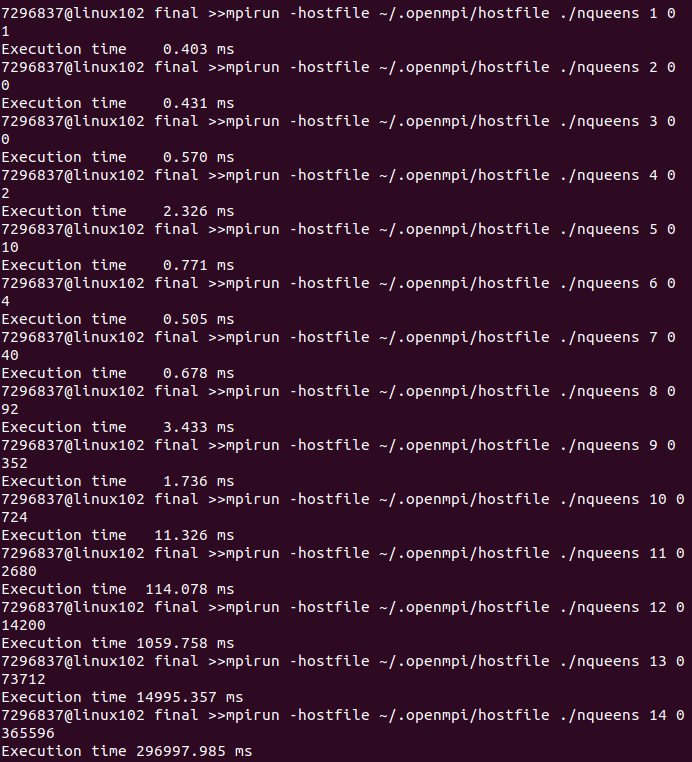
\includegraphics[width=0.5\textwidth]{solutions.png} 
    \caption{Number of solutions till n=14}
    \label{fig:solutions}
\end{figure}

% • Description of what you have submitted: Makefile, external functions, main, 
% etc.
% • Data in form of spreadsheets, graphs etc.
\section{Files Submitted}
\begin{itemize}
    \item \texttt{final.pdf}
    \item \texttt{makefile}
    \item \texttt{nqueens.C}
    \item \texttt{final.xlsx}
    \item \texttt{latex/}
\end{itemize}

\end{document}